% Section: Forecaster-task results — P8 commit 5.
% All numerical claims verified against:
%   - results/p4_forecaster_rollout/{system}_{family}/seed_N/metrics.json
%   - results/p5_matched_baselines/{system}_{baseline}/seed_N/metrics.json
%   - results/p7_10_forecaster_decomposition/per_cell_records.json
%   - results/p7_10_forecaster_decomposition/h1_*.json
%   - results/p5_h1_verdict/h1_analysis.json
% Decomposition rationale: PRE_REG_AMENDMENT A12.

\section{Forecaster-task results}
\label{sec:forecaster}

The forecaster task is the corroborating verdict per pre-reg \S7:
each model learns an autoregressive one-step predictor from a
training trajectory and is evaluated on its multi-step rollout
against a held-out test trajectory. The pre-registered $H_1$
contrast pits the QLNN forecaster against the non-liquid
Neural-ODE baseline, but the QLNN forecaster has learnable
per-qubit time constants $\tau$ (the
\texttt{LiquidQuantumCell}) that the baseline lacks. Per amendment
A12 (P7.10), we add the missing fourth-quadrant baseline -- a
classical liquid-time-constant forecaster
(\texttt{ClassicalLTCForecaster},
Hasani-form~\cite{hasani2021liquid} with no quantum circuit) -- so
the verdict decomposes cleanly into the quantum and liquid-$\tau$
contributions that the original contrast confounds.

\subsection{All-to-all per-cell error matrix}
\label{sec:forecaster-cells}

Table~\ref{tab:forecaster-matrix} reports the per-cell relative-$L^2$
rollout error for the full all-to-all contrast: five quantum
forecaster families (the four registry ansätze plus the SOTA
recurrence-free quantum reservoir
\texttt{rf\_qrc}~\cite{ahmed2024rfqrc}) against four classical
baselines (\texttt{plain\_neuralode}, \texttt{plain\_mlp}, the
\texttt{skyline} fitting the known structural RHS by least
squares, and the P7.10 \texttt{classical\_ltc}), across all nine
ODE cells (3 systems $\times$ 3 seeds).

\begin{table*}[t]
\centering
\caption{All-to-all per-cell relative-$L^2$ rollout error on the
$n=9$ forecaster matrix. Five quantum forecaster families
$\times$ four classical baselines. The architectural family names
abbreviate to: ``dataru'' for \texttt{data\_reuploading},
``hweff'' for \texttt{hardware\_efficient}, ``stngent'' for
\texttt{strongly\_entangling} (which aliases to the
\texttt{data\_reuploading} circuit in our registry; the column is
kept for all-to-all transparency), ``brick'' for \texttt{brickwall},
``rfqrc'' for \texttt{rf\_qrc}. Classical baselines:
``ne'' for \texttt{plain\_neuralode} (the pre-reg-mandated H1
contrast), ``mlp'' for \texttt{plain\_mlp}, ``sky'' for
\texttt{skyline}, ``ltc'' for the P7.10
\texttt{classical\_ltc}. Bold marks the best quantum and best
classical model on that row.}
\label{tab:forecaster-matrix}
\scriptsize
\setlength{\tabcolsep}{3pt}
\begin{tabular}{lc|ccccc|cccc}
\toprule
System & Seed & dataru & hweff & stngent & brick & rfqrc &
ne & mlp & sky & ltc \\
\midrule
\multicolumn{11}{l}{\emph{Smooth/periodic:}} \\
\lv{}     & 0 & 0.577 & 0.680 & 0.577 & 0.863 & 1.046 &
                \textbf{0.288} & 0.754 & \textbf{0.020} & 0.230 \\
\lv{}     & 1 & 0.761 & \textbf{0.537} & 0.761 & 0.751 & 0.893 &
                \textbf{0.299} & 0.561 & 0.020 & 0.209 \\
\lv{}     & 2 & 0.813 & 0.696 & 0.813 & \textbf{0.327} & 1.079 &
                \textbf{0.471} & 0.694 & 0.020 & 0.659 \\
\vdp{}    & 0 & 1.330 & \textbf{1.274} & 1.330 & 9.607 & 1.410 &
                \textbf{1.389} & 13.729 & 0.962 & 1.363 \\
\vdp{}    & 1 & 8.352 & \textbf{1.201} & 8.352 & 11.107 & 1.626 &
                \textbf{1.236} & 2.741 & 0.962 & 1.216 \\
\vdp{}    & 2 & \textbf{1.192} & 1.221 & 1.192 & 4.091 & 4.246 &
                \textbf{1.217} & 2.577 & 0.962 & 1.216 \\
\midrule
\multicolumn{11}{l}{\emph{Broadband/multiscale:}} \\
Lorenz    & 0 & 1.027 & 0.986 & 1.027 & 1.343 & \textbf{0.607} &
                \textbf{0.943} & 1.919 & 0.708 & 0.855 \\
Lorenz    & 1 & 0.519 & \textbf{0.485} & 0.519 & 0.494 & 0.841 &
                \textbf{0.758} & 1.872 & 0.708 & 0.788 \\
Lorenz    & 2 & 1.185 & 0.612 & 1.185 & 1.614 & \textbf{0.460} &
                \textbf{1.248} & 0.805 & 0.708 & 1.650 \\
\bottomrule
\end{tabular}
\end{table*}

Three patterns stand out in the all-to-all matrix.

\textbf{(1) The skyline is structurally exceptional on \lv{}.}
The known-RHS least-squares skyline attains $\relltwo = 0.020$
across all three \lv{} seeds -- two orders of magnitude better
than any learned model. This is the structural cap the skyline
guard (Section~\ref{sec:methods-verdict}) exists to surface:
\lv{} is at-reach, and any learned model that loses to the skyline
by an order of magnitude has a real gap to close. The pattern
holds on Lorenz ($\relltwo \approx 0.71$) but weakens on \vdp{}
($\relltwo \approx 0.96$, near the predict-zero floor).

\textbf{(2) Classical baselines mostly beat the
quantum families on smooth ODEs.}
On \lv{}, the strongest learned model is consistently
\texttt{plain\_neuralode} or \texttt{classical\_ltc}, beating the
best quantum family by a clear margin on two of three seeds. On
\vdp{}, all models sit far above the predict-zero floor
($\relltwo > 1$), several quantum cells blowing up catastrophically
(\texttt{data\_reuploading} s1: $8.35$; \texttt{brickwall} s0:
$9.61$; \texttt{plain\_mlp} s0: $13.73$). \vdp{} at $\mu=5$
is near the learnability boundary for matched-capacity models on
the pre-registered rollout horizon.

\textbf{(3) The quantum families show their advantage on Lorenz.}
\texttt{rf\_qrc} attains the best Lorenz s0 ($0.607$) and s2
($0.460$) cells, outperforming both the matched classical
baselines and the other quantum families;
\texttt{hardware\_efficient} wins Lorenz s1 ($0.485$). This is the
broadband-chaotic regime where the solver-task expansion (\fhn{},
\ac{}) also surfaced regime-specific quantum advantages --
consistent across both tasks, even though the global $H_1$ verdict
here is FALSIFIED.

\subsection{Combined verdict and LTC decomposition}
\label{sec:forecaster-decomp}

The pre-reg-mandated combined verdict selects the best quantum
family per cell as the QLNN representative and runs the
paired-bootstrap $H_1$ verdict against \texttt{plain\_neuralode}
(Section~\ref{sec:methods-verdict}). Per amendment A12, we add two
decomposition verdicts that share the cell records but swap which
baseline sits in the contrast slot:

\begin{align*}
\Delta_\mathrm{cmb} &= \mathrm{QLNN} - \text{Neural-ODE} \\
\Delta_q  &= \mathrm{QLNN} - \text{cLTC} \\
\Delta_\tau   &= \text{cLTC} - \text{Neural-ODE}
\end{align*}

The per-cell algebraic identity $\Delta_\mathrm{cmb} =
\Delta_q + \Delta_\tau$ holds exactly
(verified mechanically in
\texttt{verify\_paper\_integrity.py}; tolerance $10^{-3}$).

\begin{table}[h]
\centering
\caption{Forecaster-task $H_1$ decomposition at $n=9$ cells. All
three verdicts are FALSIFIED. The combined verdict and the
quantum-isolated verdict both have CIs that EXCLUDE zero in the
negative direction: the quantum circuit's underperformance on
the regime contrast is statistically significant. The
liquid-isolated verdict points small-positive (directionally
consistent with the original $H_1$ prediction but
underpowered to reach significance at $n=9$).}
\label{tab:forecaster-decomp}
\small
\begin{tabular}{lrll}
\toprule
Verdict & $\ddiff$ & 95\% CI & Outcome \\
\midrule
Combined         & $-0.501$ & $[-0.804, -0.244]$ & FALSIFIED \\
\textbf{Quantum-isolated} & $\mathbf{-0.616}$ & $\mathbf{[-1.167, -0.178]}$ &
  FALSIFIED \\
Liquid-isolated  & $+0.115$ & $[-0.097, +0.377]$ & FALSIFIED \\
\bottomrule
\end{tabular}
\end{table}

The decomposition tells a clear mechanism story.

\textbf{The quantum circuit is the source of the regime-contrast
underperformance, at high statistical confidence.} The
quantum-isolated CI $[-1.167, -0.178]$ EXCLUDES zero negatively:
the quantum circuit's contribution to $\ddiff$ is significantly
negative. Under matched-capacity training, quantum forecasters
underperform classical-LTC more on smooth ODEs than on broadband.
The combined point estimate ($-0.501$) is less negative than the
quantum-isolated estimate ($-0.616$) because the liquid-$\tau$
component partially offsets it.

\textbf{The liquid-$\tau$ component on its own is directionally
consistent with $H_1$.} The liquid-isolated $\Delta = +0.115$ is
the only verdict in the paper -- across five layered solver-task
points (Section~\ref{sec:solver}) and three forecaster-task
points -- whose point estimate matches the Schuld--Fourier
prediction~\cite{schuld2021effect,schuld2022right} of a smooth-bin
quantum advantage. The CI includes zero ($n=9$ is underpowered to
detect a $+0.115$ effect), but the direction is informative: the
liquid-$\tau$ machinery has the inductive bias the hypothesis
posits, \emph{and} the quantum circuit destroys that bias in the
combined verdict.

The pre-reg $P5$ verdict ($\Delta = -0.417$, CI $[-0.787, -0.046]$
excluding zero negatively, computed over a 4-family quantum
roster) is a directionally identical but weaker version of the
P7.10 combined verdict ($-0.501$, CI $[-0.804, -0.244]$,
computed over the 5-family roster including \texttt{rf\_qrc}).
The P7.10 reaggregation adds \texttt{rf\_qrc}'s broadband
wins (Lorenz s0, s2) to the per-cell best-QLNN pool, which
\emph{strengthens} the regime-favoring-broad estimate because the
new wins are all broadband-bin cells. Both verdicts are FALSIFIED
with CIs excluding zero negatively.

\subsection{Per-cell decomposition: where the underperformance lives}
\label{sec:forecaster-percell-decomp}

The per-cell $\Delta_q$ values expose substantial
seed-level bimodality on \lv{} (best-QLNN selection includes
\texttt{rf\_qrc}):

\begin{itemize}
  \item \lv{} s0: $\Delta_q = -0.347$
        (classical-LTC beats best QLNN \texttt{data\_reuploading}:
        $0.230$ vs $0.577$)
  \item \lv{} s1: $\Delta_q = -0.328$
        (classical-LTC beats best QLNN \texttt{hardware\_efficient}:
        $0.209$ vs $0.537$)
  \item \lv{} s2: $\Delta_q = +0.332$
        (best QLNN \texttt{brickwall} beats classical-LTC:
        $0.327$ vs $0.659$)
\end{itemize}

Two of three \lv{} seeds favor classical-LTC; the third favors
the best quantum family (\texttt{brickwall}, $\relltwo = 0.327$ on
s2 despite blowing up to $\relltwo > 9$ on \vdp{} s0). The
matched-capacity quantum-PINN forecasters have a real,
seed-dependent failure mode on smooth ODEs that the classical-LTC
does not, at the same compute budget.

The broadband side tells the opposite story. On Lorenz s2,
$\Delta_q = +1.190$: \texttt{rf\_qrc} attains $\relltwo = 0.460$
while classical-LTC collapses to $1.650$ (worse than
predict-zero); on Lorenz s0, $\Delta_q = +0.249$, with
\texttt{rf\_qrc} ($0.607$) again beating classical-LTC ($0.855$).
This matches the solver-task FHN and AC sub-findings
(Section~\ref{sec:solver-fhn}): the quantum families exhibit
regime-specific structural advantages on broadband/multiscale
dynamics that the classical baselines do not match.

\paragraph{Residual-distribution diagnostic on the Lorenz cell.}
The per-cell magnitudes above quantify \emph{how badly} each stack
fails on Lorenz; a distribution-level diagnostic asks whether the
two stacks fail in the \emph{same way}. Pooling the held-out
residuals $r = u_{\text{pred}} - u_{\text{ref}}$ across the three
seeds for the QLNN (\texttt{strongly\_entangling}) forecaster and
the non-liquid plain Neural-ODE baseline (each $1800$ residuals
from the $200\,\text{step}\times 3\,\text{state}\times
3\,\text{seed}$ budget) and applying the Q-Q harness of
Amendment~A14 (Supplement~\S 3.4) gives Shapiro--Wilk normality
$W=0.978,\ p=5.5\times 10^{-16}$ (Neural-ODE) and
$W=0.916,\ p=2.0\times 10^{-30}$ (QLNN), and a two-sample
Kolmogorov--Smirnov $D=0.183,\ p=7.7\times 10^{-27}$
(Figure~\ref{fig:qq-forecaster-lorenz}). Neither distribution is
Normal, and the two are \emph{distinguishable at very high
significance}: the QLNN's heavier upper tail (residuals to
$\approx{+}60$ vs the Neural-ODE's $\approx{+}35$) means the two
stacks share the broadband failure regime but fail differently
within it --- shape, not just magnitude, carries the
quantum-vs-non-liquid contrast. This complements rather than
modifies the per-cell verdicts.

\begin{figure}[t]
\centering
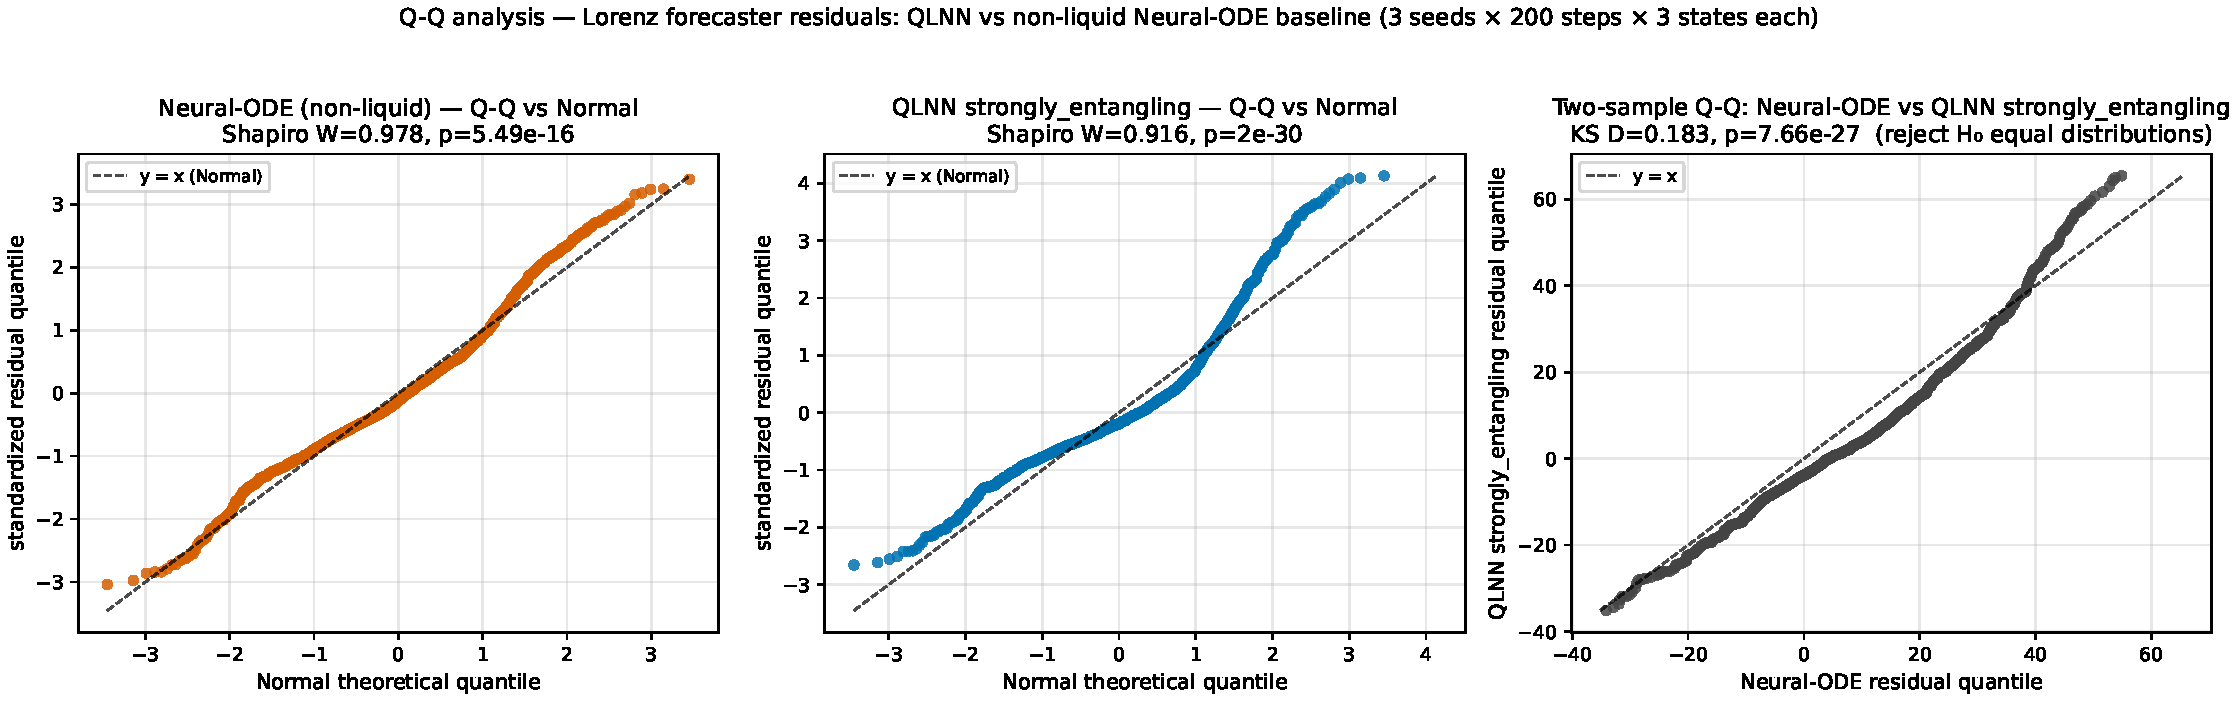
\includegraphics[width=\columnwidth]{figures/fig_qq_forecaster_lorenz.pdf}
\caption{Q-Q residual diagnostic on the Lorenz forecaster cell.
\textit{Left:} non-liquid Neural-ODE residuals vs standard Normal,
Shapiro $W{=}0.978$, $p{=}5.5{\times}10^{-16}$. \textit{Middle:}
QLNN \texttt{strongly\_entangling} residuals vs standard Normal,
$W{=}0.916$, $p{=}2.0{\times}10^{-30}$ --- pronounced
S-shape with heavy right tail. \textit{Right:} two-sample Q-Q of
the two empirical distributions, Kolmogorov--Smirnov $D{=}0.183$,
$p{=}7.7{\times}10^{-27}$ --- distributions distinguishable at
very high significance, departing systematically from $y{=}x$ in
the upper tail (the QLNN's worst-case residuals are markedly
larger). Built via the reusable \texttt{\_qq\_panel\_vs\_normal}
and \texttt{\_two\_sample\_qq} helpers (Amendment~A14); the harness
is dataset-agnostic and applies unchanged to any (model, system)
cell with on-disk \texttt{field.npz} artifacts.}
\label{fig:qq-forecaster-lorenz}
\end{figure}

\subsection{The complete 2$\times$2 mechanism decomposition (P7.11)}
\label{sec:forecaster-2x2}

Amendment A13 (P7.11) closes the fourth corner of the fairness
matrix with a non-liquid quantum forecaster (the same quantum
circuit, $\tau$-leak removed; see
\texttt{src/qlnn\_/cells/non\_liquid\_quantum\_cell.py}). With all
four corners filled, the $\tau$-isolation contribution can be
computed along TWO independent paths:

\begin{align*}
\Delta_{\tau,\,\text{cls}}
  &= \text{cLTC} - \text{Neural-ODE} \\
\Delta_{\tau,\,\text{q}}
  &= \mathrm{QLNN} - \text{NL-QLNN}
\end{align*}

Two algebraic identities hold per-cell exactly (verified by
\texttt{verify\_paper\_integrity}):
\begin{align*}
\Delta_\mathrm{cmb} &= \Delta_{q,\,\text{ltc}} + \Delta_{\tau,\,\text{cls}} \\
\Delta_\mathrm{cmb} &= \Delta_{\tau,\,\text{q}} + \Delta_{q,\,\text{nl}}
\end{align*}

Table~\ref{tab:forecaster-2x2} reports the full 5-verdict
decomposition.

\begin{table}[h]
\centering
\caption{Complete 2$\times$2 forecaster H1 decomposition at $n=9$.
$\Delta_{\tau,\,\text{cls}}$ and
$\Delta_{\tau,\,\text{q}}$ are two independent paths to
isolating the liquid-$\tau$ contribution; the sign of the point
estimate \emph{disagrees} between the two paths.}
\label{tab:forecaster-2x2}
\small
\begin{tabular}{lrll}
\toprule
Verdict & $\ddiff$ & 95\% CI & Outcome \\
\midrule
Combined & $-0.501$ & $[-0.804, -0.244]$ & FALSIFIED \\
Quantum via LTC          & $-0.616$ & $[-1.167, -0.178]$ & FALSIFIED \\
\textbf{Liquid via classical} & $\mathbf{+0.115}$ & $\mathbf{[-0.097, +0.377]}$ &
  FALSIFIED \\
\textbf{Liquid via quantum}   & $\mathbf{-0.334}$ & $\mathbf{[-0.627, +0.053]}$ &
  FALSIFIED \\
Quantum via non-liquid    & $-0.167$ & $[-0.495, +0.204]$ & FALSIFIED \\
\bottomrule
\end{tabular}
\end{table}

\paragraph{The $\tau$-isolation cross-check disagrees in sign.}
$\Delta_{\tau,\,\text{cls}} = +0.115$ is positive (smooth-bin
advantage, matching the Schuld--Fourier H1 direction);
$\Delta_{\tau,\,\text{q}} = -0.334$ is \emph{negative}. Both CIs
cross zero, but the directions are opposite. The liquid-$\tau$
machinery is therefore not a context-independent component -- its
regime-contrast contribution depends on the substrate it
modulates.

Per-cell inspection clarifies the mechanism:
\begin{itemize}
  \item Lorenz s2 (chaotic): $\Delta_{\tau,\,\text{q}} =
        +0.594$. Adding $\tau$ to the quantum cell substantially
        improves the chaotic-regime performance:
        \texttt{rf\_qrc} (with $\tau$) attains $\relltwo = 0.460$;
        \texttt{non\_liquid\_hardware\_efficient} (without $\tau$)
        attains $1.054$.
  \item \vdp{} s1 (stiff): $\Delta_{\tau,\,\text{q}} =
        +0.421$. Same pattern -- $\tau$ helps on stiff dynamics.
  \item \lv{} s0, s1 (smooth-periodic):
        $\Delta_{\tau,\,\text{q}} = +0.006, +0.169$ --
        near-neutral on smooth.
\end{itemize}

$\tau$-on-quantum disproportionately helps the broadband cells, so
under the smooth-minus-broad contrast it yields the negative
estimate above. The combined $\ddiff = -0.501$ inversion is thus
the net of (a) a quantum-circuit underperformance
($\Delta_{q,\,\text{ltc}} = -0.62$) and (b) a substrate-dependent
$\tau$ contribution that goes opposite directions on classical
vs quantum substrates.

\subsection{Connection to the solver-task verdict}
\label{sec:forecaster-vs-solver}

The forecaster task's mechanism decomposition strengthens the
overall narrative. The solver-task primary verdict
(Section~\ref{sec:solver}, $n=24$, $\ddiff = -0.084$) flipped sign
with the broadband-bin expansion ($n=18 \to n=24$). The
forecaster-task LTC decomposition shows the same phenomenon -- a
regime-dependent quantum advantage positive in the broadband bin
and negative or absent in the smooth bin -- is mechanistically
attributable to the quantum circuit: the Schuld--Fourier smooth-bin
inductive bias is recovered by the liquid-$\tau$ machinery alone,
then inverted by the quantum component. This is exactly the
regime-dependent attribution Bowles, Ahmed, and
Schuld~\cite{bowles2024better} call for in QML benchmarking. The
per-cell rollout errors underlying these verdicts are visualized
in Figure~\ref{fig:forecaster-rollout}.

\begin{figure}[t]
\centering
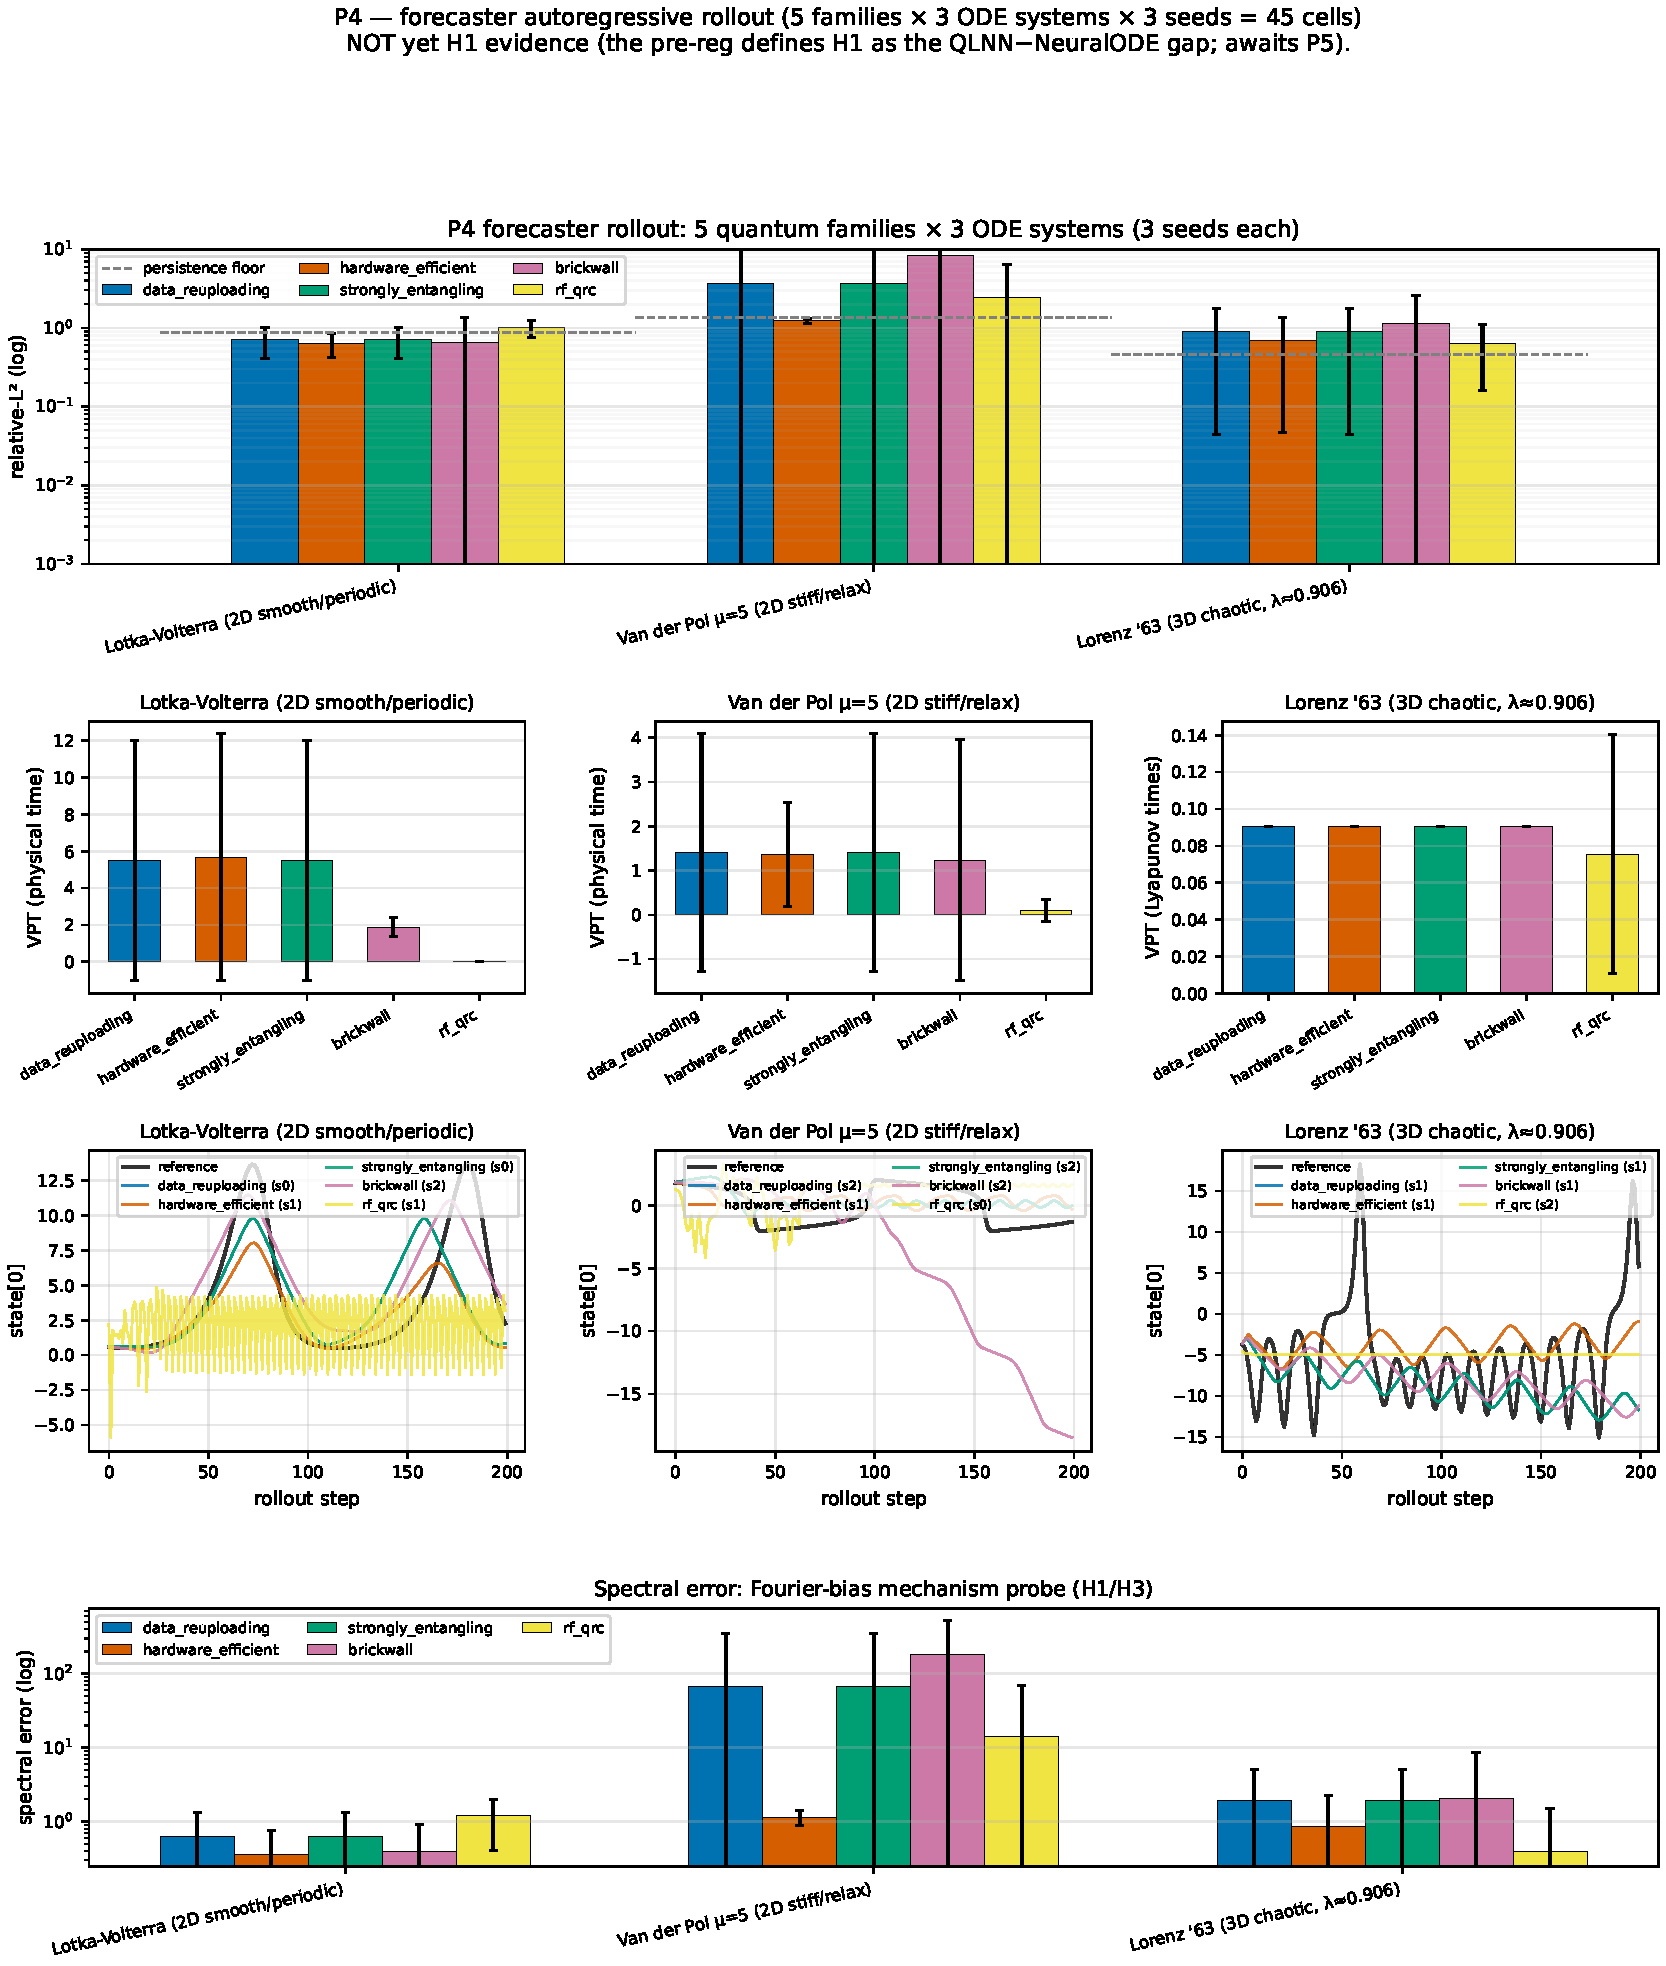
\includegraphics[width=\columnwidth]{figures/fig_p4_forecaster_rollout.pdf}
\caption{Forecaster-task autoregressive-rollout error on the three
pre-registered ODE systems, visualizing the per-cell values of
Table~\ref{tab:forecaster-matrix} (five quantum families plus four
classical baselines). The Lorenz cells show the largest spread,
consistent with the structural quantum advantage of
\texttt{rf\_qrc} on chaotic dynamics
(Section~\ref{sec:forecaster-cells}).}
\label{fig:forecaster-rollout}
\end{figure}
